\documentclass{gescons}

\genre {Entrevista}
\author{Michel Chad}
\title{Megapensenes Trivocabulares Pró-evolutivos}

\begin{document}
    \makeentrevistatitle
    \coverart{back/Michel_Chad}

    \begin{multicols}{2}


%\noindent\includegraphics[width=9cm, height=7cm]{example-image} 

\begin{center}
    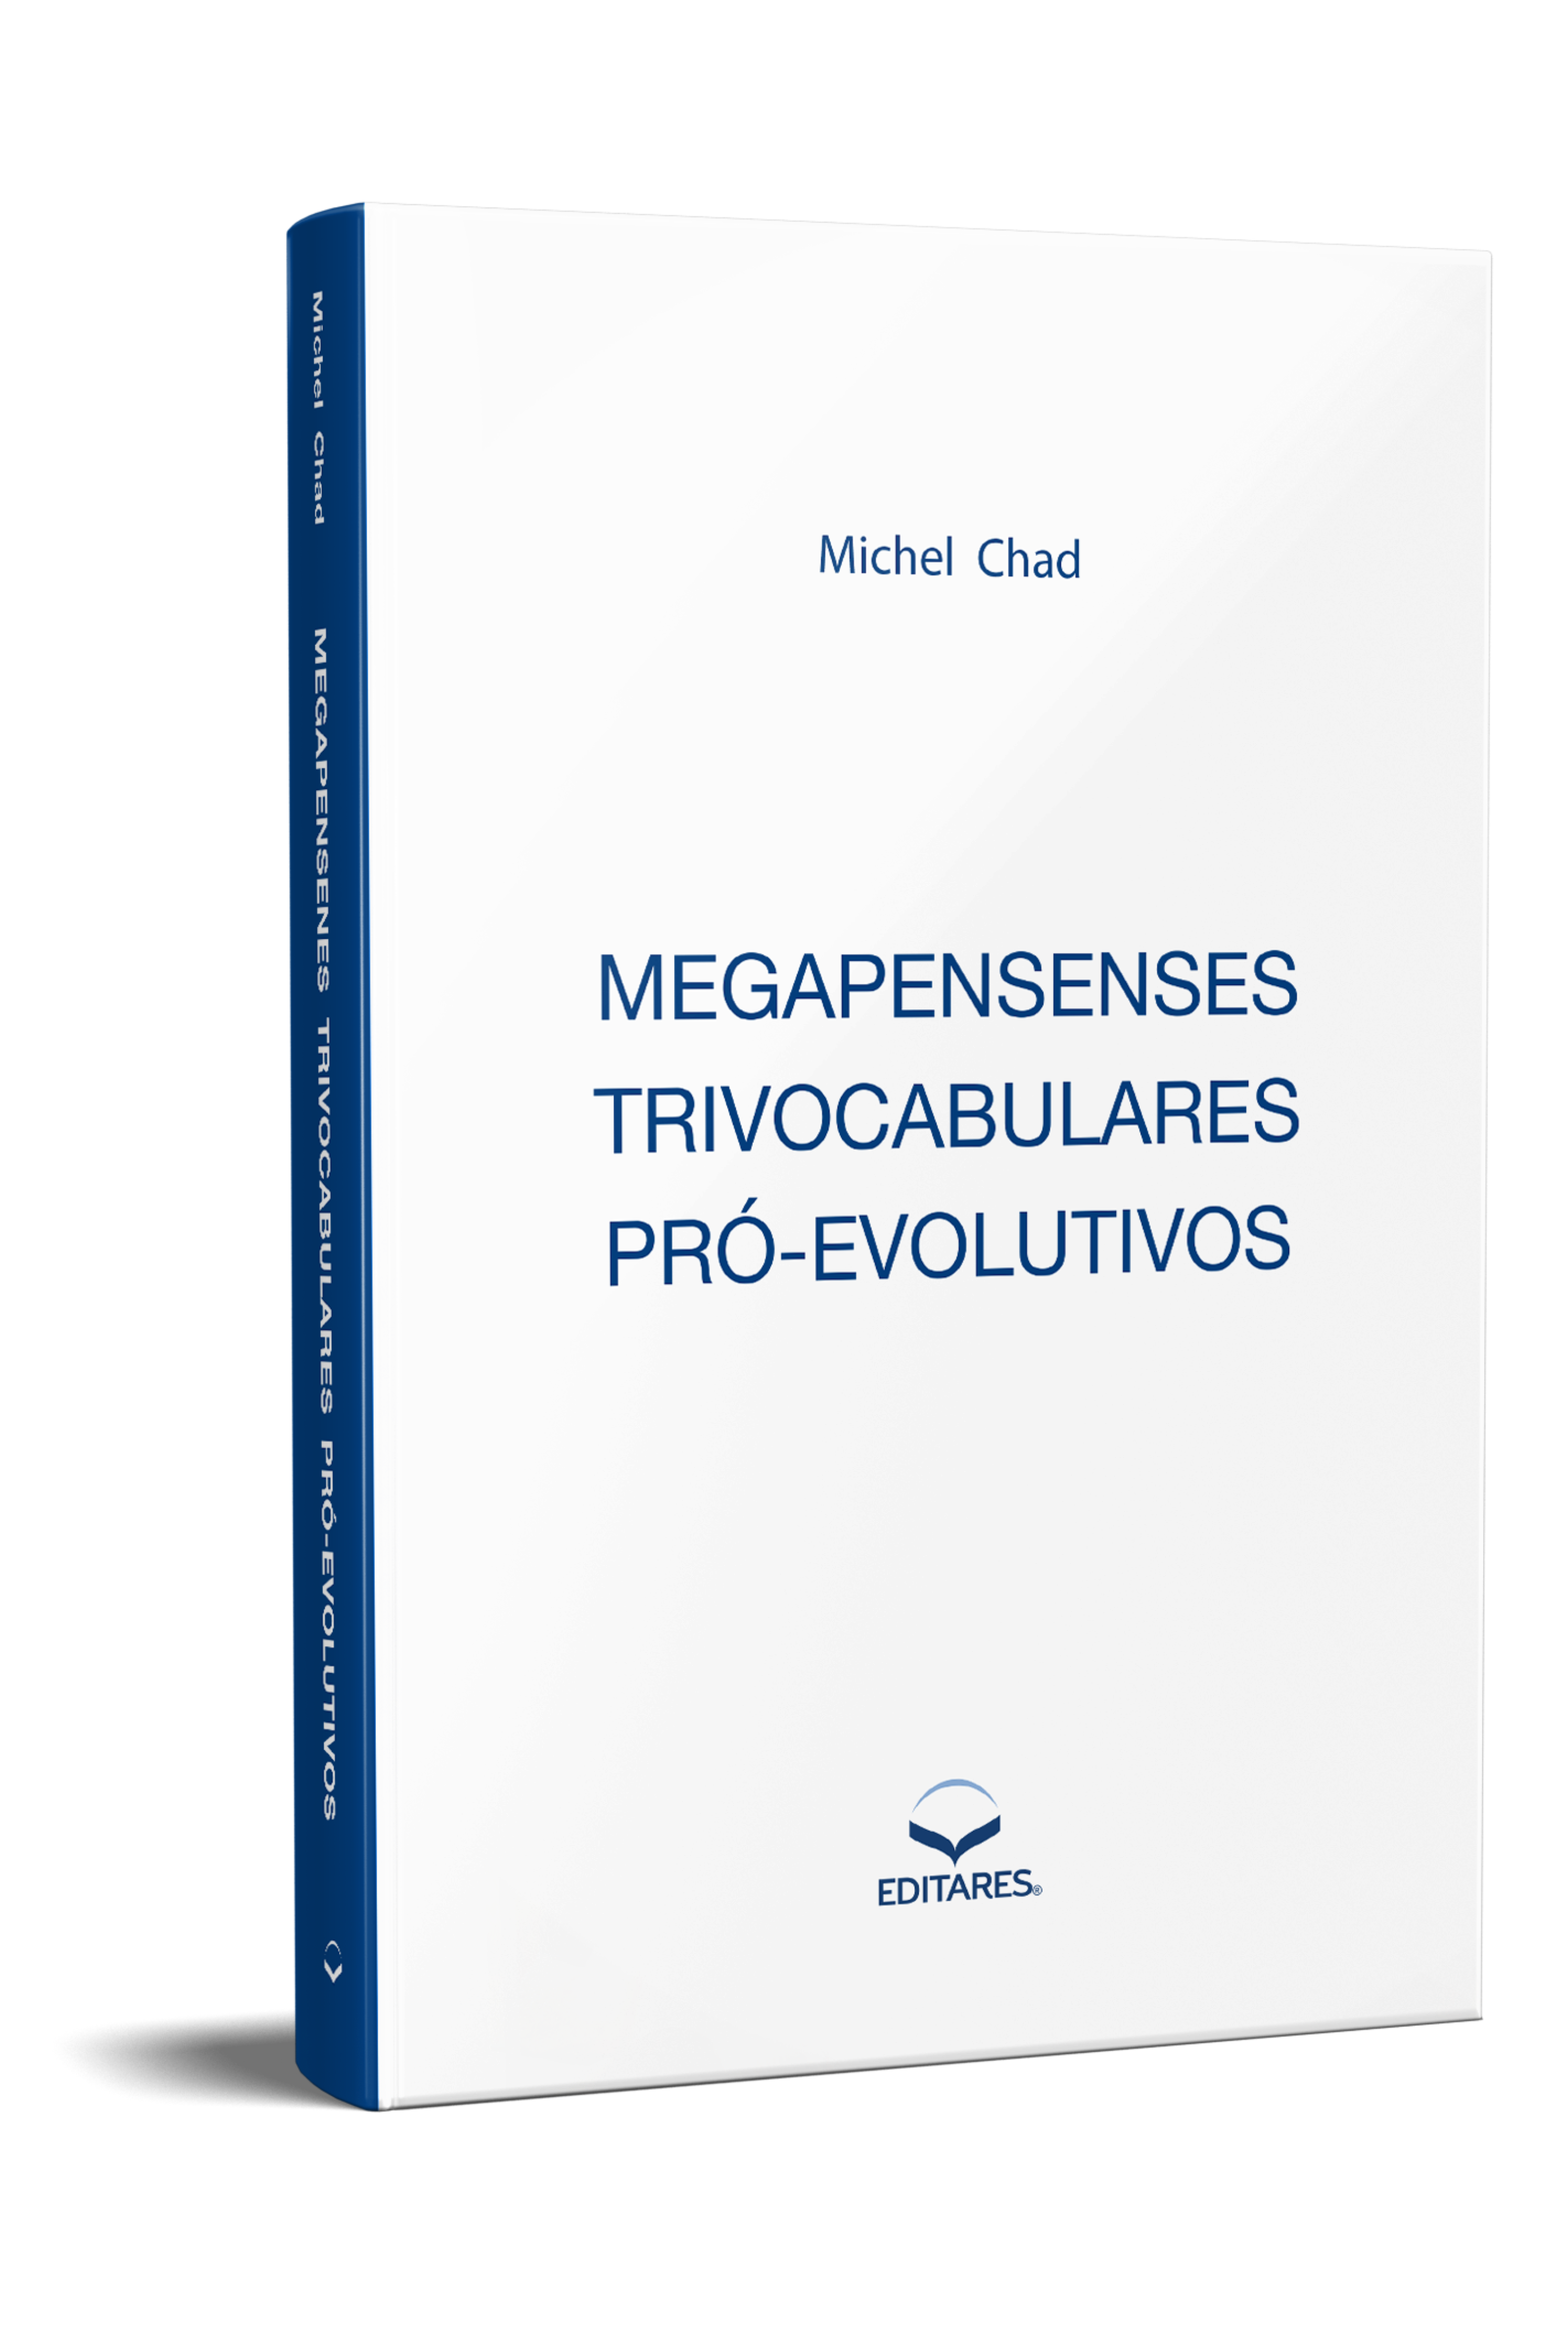
\includegraphics[width=8cm]{articles/entrevista/mockups/Michel-Chad.png}
\end{center}

\textbf{1.       Qual foi a motivação para a escrita da obra? Por que a definição deste tema para publicação de um livro?}

Sou voluntário do IIPC desde 1996. Desde que Waldo Vieira apresentou esta técnica em um curso avançado ministrado em São Paulo, comecei a estudar os megapensenes trivocabulares e elaborar meus próprios. 

Nesta época participava do \textit{Grupo de Pesquisa da Conscienciologia} (GPC) do livro de Waldo Vieira,  \textit{700 Experimentos da Conscienciologia.} Tínhamos encontros semanais de estudo prévio de 2 capítulos do tratado e, na reunião, criávamos uma pensata sobre cada um dos capítulos. Posteriormente, o desafio era formular uma nova frase síntese juntando as duas anteriores. Diversas vezes criamos megapensenes trivocabulares nesta tarefa. 

Talvez pela minha formação em Engenharia Química, o processo de confecção das pensatas trivocabulares e suas 200 fórmulas apresentadas no
\textit{Manual de Megapensenes Trivocabulares,} de Waldo Vieira,  fascinou-me. Pela leitura crítica deste material, busquei aprender e utilizar, na confecção dos meus megapensenes, todas as fórmulas descritas. Inclusive no meu livro proponho 6 fórmulas inéditas criadas por mim.

Outra gescon que serviu como modelo  para minha obra, foi o livro \textit{Megapensenes Trivocabulares da Interassistencialidade,} de Aline Niemeyer, publicado em 2016.

Participei do curso Técnica de Mais 1 ano de Vida Intrafísica, em 2016 e 2017,  ministrado pelo CEAEC, no qual uma das minhas metas foi a escrita e publicação de uma obra com megapensenes trivocabulares. Meta finalmente cumprida em 2024.

\textbf{2.       Quais foram as principais percepções, intra e extrafísicas, durante a pesquisa e a escrita da obra? E posterior ao lançamento?}

Penso que entre as gescons que me propus no meu curso intermissivo, uma delas está relacionada com a produção de neopensatas trivocabulares. 

\begin{pullquote}
    ``Penso que entre as gescons que me propus no meu curso intermissivo, uma delas está relacionada com a produção de neopensatas trivocabulares.''
\end{pullquote}

\textbf{3.       Qual o maior aprendizado com a escrita desta obra?}

Cito entre os benefícios no estudo e elaboração dos megapensenes trivocabulares: ampliação dos diversos dicionários cerebrais, inclusive o analógico; aprimoramento do atributo da associação de ideias; aprofundamento no pensar; comunicação interassistencial sintética; criação do hábito de compor sínteses; desassédio mental; desenvolvimento da criticidade; facilitação da criação e compreensão de neologismos; flexibilidade pensênica; hábito das ponderações das verpons; indução da criatividade.


\textbf{4.       O que poderia dizer como incentivo para que mais pesquisadores invistam na publicação de obras conscienciológicas?}

Finalizo agradecendo a todas as consciências envolvidas neste projeto sugerindo aos interessados estudarem a fundo as 200 fórmulas apresentadas no livro e desenvolverem os seus próprios megapensenes trivocabulares. Elabore neopensatas trivocabulares.


\begin{pullquote}
``Elabore neopensatas trivocabulares.''
\end{pullquote}
    
    \end{multicols}
\end{document}


